\section{Summary of Papers}
\label{sec:summary}

\subsection{AutoNER}
AutoNER \cite{autoner} is the recent SOTA in domain-specific NER. It has two contributions: Fuzzy LSTM CRF and Tie-or-Break scheme.
\\

\noindent\textbf{Tie-or-Break Scheme}
In a sentence, predict whether two words should be tied together to form one phrase or broken apart. Now, between every to 'breaks' you have a potential named entity. Predict its type ('None' being the type that it's not a named entity).

Training data for these phrases comes from another paper of the same group \cite{autophrase} which uses unsupervised methods to extract interesting phrases from a large corpus.
\\

\noindent\textbf{Fuzzy LSTM CRF}
Have to read about CRF and how they work. 
\begin{enumerate}
	\item Neither BERT nor ELMO use CRF and both report SOTA results on NER.
	\item Need to check if CRFs work for domain specific case? If so, why?
\end{enumerate}

They also introduce a training mechanism which models the noise in supervision.
Let $v_i$ be the vector for a phrase (constructed using concatenation of beginning and ending word). Pass it through a softmax layer to get 

\[
	p(t_j|v_i) = \frac{e^{t_j^Tv_i}}{\sum_{k}{e^{t_k^Tv_i}}}
\]

Usually, you would now take a cross-entropy loss. But since a word can belong to multiple types, define
\[
	\hat{p}(t_j|v_i) = \frac{\delta(s_i \in t_j) e^{t_j^Tv_i}}{\sum_{k}{\delta(s_i \in t_k)e^{t_k^Tv_i}}}
\]

where $\delta$ is a boolean function which checks whether the span $s_i$ is ever marked with type $t_j$ in distant supervision.

Now take cross-entropy loss between $p$ and $\hat{p}$.

The only difference between $\hat{p}$ and $p$ is that to get $\hat{p}$ you mask the values of $p$ that are never assigned in distant supervision. 

Essentially this punishes the model if it gives any weight to those values and allows the model to learn whatever it wants for the probable types.

\reminder{Maybe there's something wrong here.} But if the above is true, the model never gets to see the true type in the current context. How will the model learn to disambiguate?


\begin{figure*}[t]
	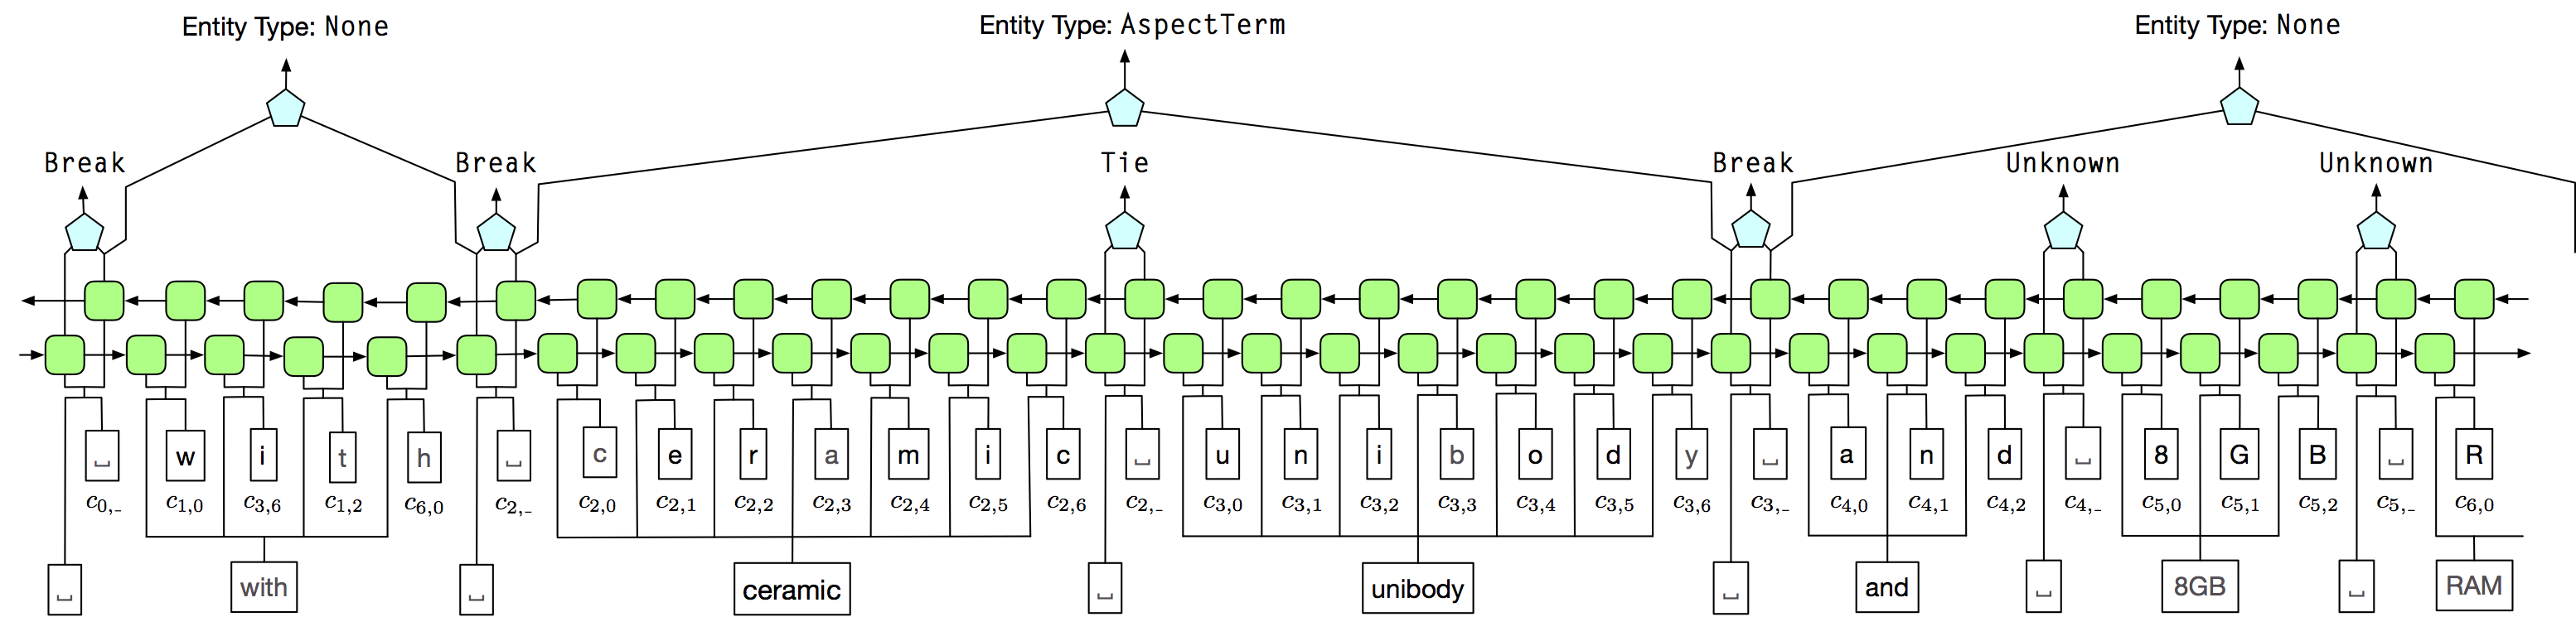
\includegraphics[scale=0.3]{images/autoner_tie_or_break.png}
	\caption{\label{fig:tie_or_break}Overview of the Tie-or-Break scheme used in AutoNER.}
\end{figure*}

\subsection{Character Level Language Modeling}
\begin{enumerate}
	\item Character level features are important for NER. For instance, first letter being capitalized implies a proper noun, names of places in North India typically end in '-pur' (like Jaipur, Raipur) etc.
	\item For char-level LM, sequence lengths become too large to be directly fed into a Transformer Network. Naive solution is to break a sequence down into shorter pieces but then you lose context. One way to retain context is to keep a \textit{memory} and use that to remember earlier parts of a sequence \cite{transformerxl}.
	\item I struggled with the code of this paper. Decided to first test the hypothesis on standard BERT and if there is potential, use it for such a character-level language model as well.
\end{enumerate}

\begin{figure*}[t]
	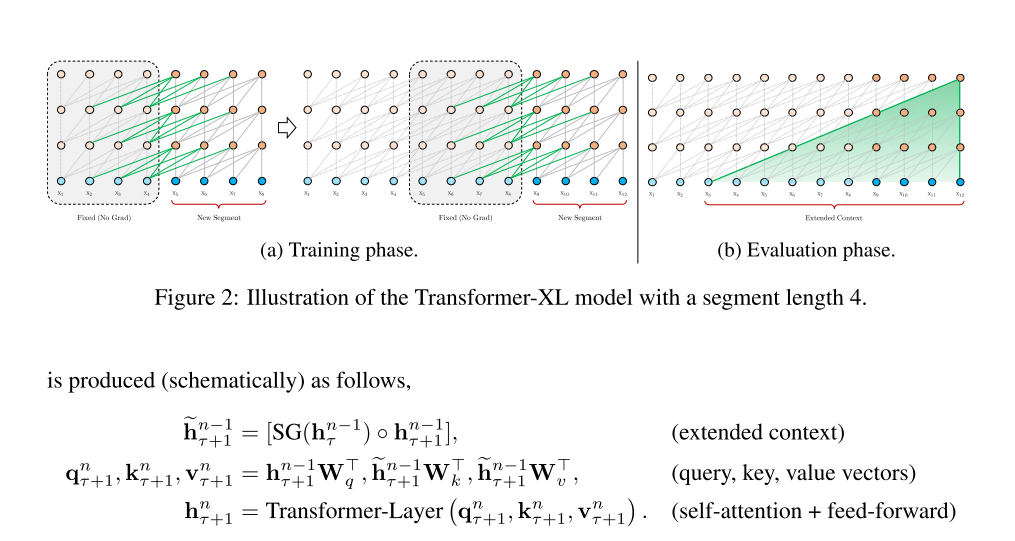
\includegraphics[scale=0.5]{images/transformerxl}
	\caption{\label{fig:transformerxl}Overview of transformer-xl which uses extended context to solve the problem of sending large sequences through Transformers.}
\end{figure*}

